\chapter{Dependency description}
\label{Chapter3}
\section{Intermodule dependency}

\begin{enumerate}
	\item [$\blacklozenge$] The Intermodule dependencies are depicted in the data flow diagram and is shown in  Fig. \ref{FIG:SWDataFlowDiag}.
	\item [$\blacklozenge$] Signals and slots are used for communication between threads and 10pps interrupt handling.
	\item [$\blacklozenge$] GUI updations at 10 Hz rate and plotting updation at 1 Hz rate.
	\item [$\blacklozenge$] The details of data formats are given in section. \ref{section:LogFormats}.
\end{enumerate}

\begin{figure}[H]
	\centering
	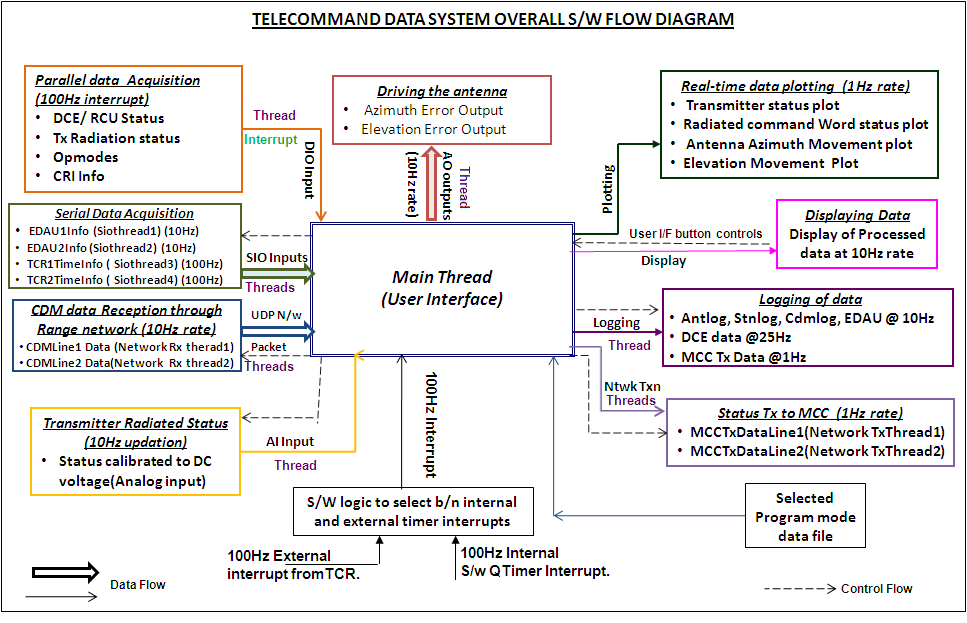
\includegraphics[width=\linewidth]{./Diagrams/SWFlowDiag.png}
	\caption{Software data flow diagram}
	\label{FIG:SWDataFlowDiag}
\end{figure}

\section{Interprocess dependencies}
Nil
\section{Data dependencies}
The data entities used in this project are grouped into the following categories:
\subsection{Input data files}
\begin{enumerate}
	
	\item [$\blacklozenge$] irig.txt file contains of the configuration parameters of IRIG-PCI cards ports for acquiring TIme data.
	\item [$\blacklozenge$] tx.txt file contains of the configuration parameters of Tx ethernet port and port numbers for acquiring data from parallel ports.
\end{enumerate}	
The details of input data configuration files are given in section. \ref{Section:InpFileFormat} and section. \ref{Section:ConnectDataPortsFormat}.

\subsection{QT  Resources}

\begin{enumerate}
	\item [$\blacklozenge$] Toolbar resource containing the buttons necessary for user interface.
	\item [$\blacklozenge$] Menubar resource containing the menu items necessary for user interface. 
	\item [$\blacklozenge$] Dialog resource for confirming selections done by the user.
	\item [$\blacklozenge$] Plotting resource for data plotting. 
	\item [$\blacklozenge$] Bitmap resource for displaying the status and updation of different parameters.
\end{enumerate}		

\subsection{System  Resources}
\begin{enumerate}
	\item [$\blacklozenge$] Memory resource.
	\item [$\blacklozenge$] Interrupt resources. 
\end{enumerate}

\subsection{Drivers}
\begin{enumerate}
	\item [$\blacklozenge$] IRIG-PCI card device drivers .
	\item [$\blacklozenge$] Qt 5.4.0 or above drivers.
	\item [$\blacklozenge$] PCI Network Ethernet drivers as a package in Red Hat Linux 7.0.
\end{enumerate}
